% ---------------------------- Preamble starts here ----------------------------

\documentclass[aspectratio=169]{beamer} %Remove [aspectratio=169] to get non-wide 4:3 slide aspect ratio

%-----------------------------------------------
% --- Set beamer theme
\usetheme{Metropolis}
\setbeamertemplate{footline}{}				% Remove automatic footer
\setbeamertemplate{navigation symbols}{}	% Comment this line to display navigation symbols

%-----------------------------------------------
% Load i2i symbol
\addtobeamertemplate{frametitle}{}{%
\begin{textblock*}{\linewidth}(0cm,7.4cm) % Replace with (0cm, 8cm) if using non-wide slide aspect
	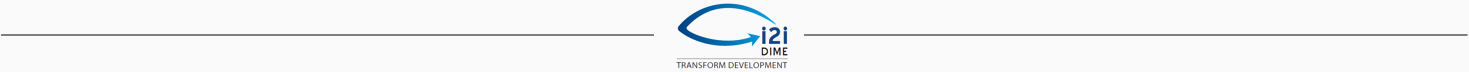
\includegraphics[width=\linewidth]{img/Footer.png}
\end{textblock*}}

\setbeamertemplate{footline}{\hfill\insertframenumber/\inserttotalframenumber}

%-----------------------------------------------
% --- Load packages
\usepackage{textpos}		% To align objects correctly
\usepackage{multicol}		% To right in multiple columns
\usepackage{color}			% To color text

%-----------------------------------------------
% --- Include link to last commit
\usepackage{xstring}
\usepackage{catchfile}

%Set this user input
\newcommand{\gitfolder}{../../../.git} %relative path to .git folder from .tex doc
\newcommand{\reponame}{worldbank/dime-github-trainings} % Name of account and repo be set in URL

%Based on this https://tex.stackexchange.com/questions/455396/how-to-include-the-current-git-commit-id-and-branch-in-my-document
\CatchFileDef{\headfull}{\gitfolder/HEAD.}{} 				%Get path to head file for checked out branch
\StrGobbleRight{\headfull}{1}[\head]						%Remove end of line character
\StrBehind[2]{\head}{/}[\branch]							%Parse out the path only
\CatchFileDef{\commit}{\gitfolder/refs/heads/\branch.}{}	%Get the content of the branch head
\StrGobbleRight{\commit}{1}[\commithash]					%Remove end of line characted

%Build the URL to this commit based on the information we now have
\newcommand{\commiturl}{\url{https://github.com/\reponame/commit/\commithash}}

%-----------------------------------------------
% --- Add your information here
\title{GitHub - Pull Request training}
\author{DIME Analytics}
\institute{DIME - The World Bank - \trainingURL{https://www.worldbank.org/en/research/dime}}
\date{\today}

\newcommand{\trainingURL}[1]{{\color{blue}\url{#1}}}

\newcommand{\traininerUsername}{kbjarkefur}
\newcommand{\repoName}{\traininerUsername/lyrics}
\newcommand{\trainingRepoURL}[1]{\trainingURL{github.com/\repoName #1}}
\newcommand{\trainerEmail}{\trainingURL{kbjarkefur@worldbank.org} }


% ---------------------------- Preamble ends here ----------------------------

\begin{document}

\begin{frame}
	\frametitle{Prerequisites}

		You can attend this presentation without these prerequisties, but you will not be able to follow along.
		
		\begin{itemize}
			\setlength\itemsep{1em}
			\item Have a WB device, for example:		
			\begin{itemize}
				\item A WB laptop or desktop
				\item A remote connection to a WB laptop or desktop				
				\item A WB VDI virtual desktop - a regular VDI is not sufficient
			\end{itemize}
			\item A WB C-account. Can be requested on eService
			\item A WB SecureID token
			\item The \textit{Microsoft Authenticator} app installed on your smart phone
		\end{itemize}
\end{frame}

\begin{frame}
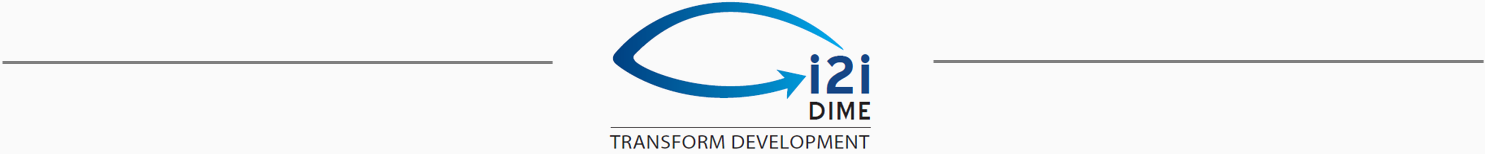
\includegraphics[width=\textwidth]{img/Header.png}
\vspace{-0.2cm}
\titlepage 	 % Opening slide, prints inform
\end{frame}


\section{WB AWS}





\begin{frame}
\frametitle{A typical WB AWS resource}

	\begin{columns}[c]
		\column{.50\textwidth} % Left column and width
		\large All WB AWS resources will be hosted in an \textit{AWS Island}
		\vspace{.7cm}\newline
		\large \textbf{Manage}: All WB AWS resources are managed through the AWS console.
		\vspace{.7cm}\newline
		\large \textbf{Access}: Any access to a WB AWS resource must go trough a gateway (gw) server
		
		\column{.50\textwidth} % Right column and width
		\begin{figure}
			\centering
			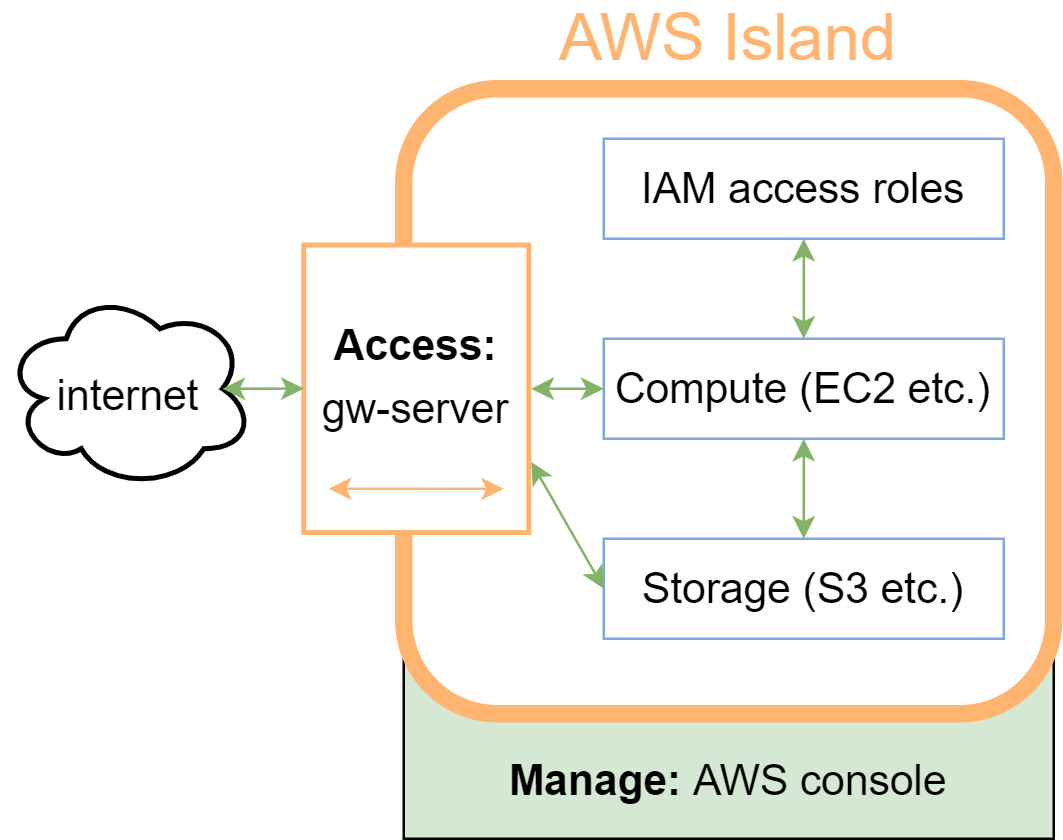
\includegraphics[width=\textwidth]{./img/wb-aws.png}
		\end{figure}

	\end{columns}
\end{frame}



\section{Manage WB AWS resources}

\begin{frame}
	\frametitle{WB AWS resource - Manage?}
	\begin{columns}[c]
		\column{.50\textwidth} % Left column and width
		We \textbf{manage} the settings of our AWS resources in the AWS console. 
		\vspace{.5cm}\newline
		Mostly relevant for ITS, but a few settings are important to us
		\vspace{.5cm}\newline
		Examples:
		\begin{itemize}
			%\setlength\itemsep{1em}
			\item Start and stop EC2 instances (cost efficiency)
			\item Manually upload files to S3 buckets
		\end{itemize}
		
		\column{.50\textwidth} % Right column and width
		\begin{figure}
			\centering
			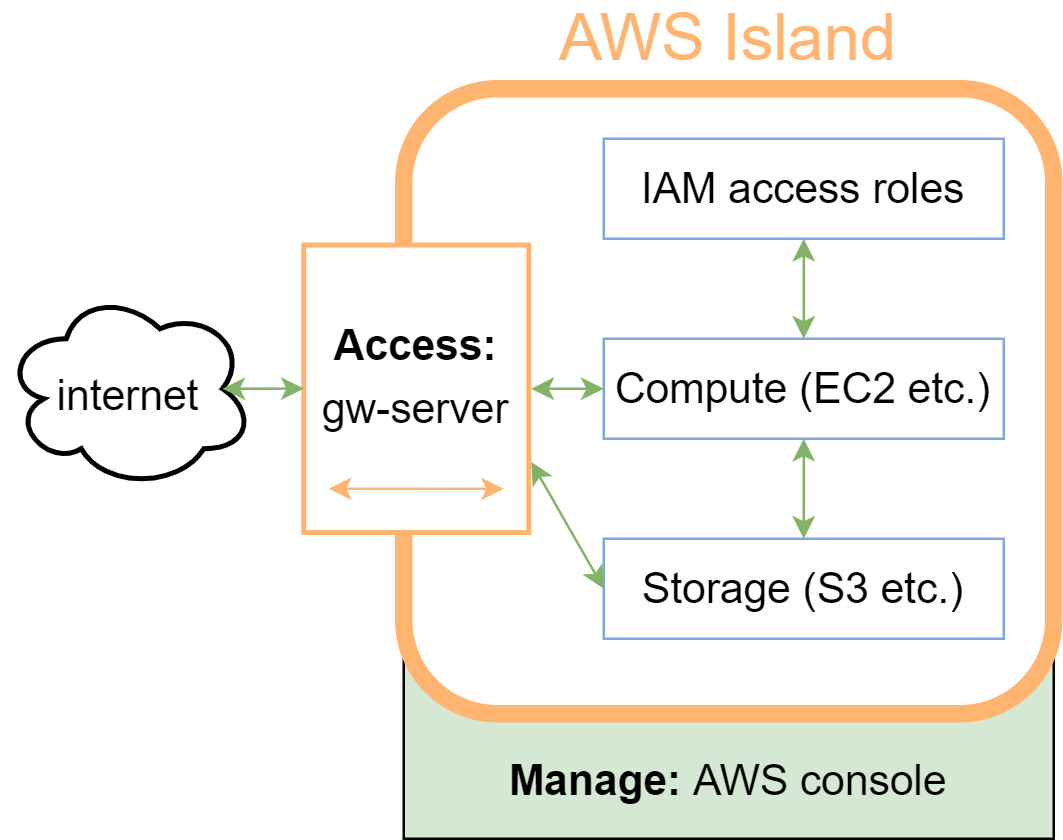
\includegraphics[width=\textwidth]{./img/wb-aws.png}
		\end{figure}
		
	\end{columns}
\end{frame}

\begin{frame}
	\frametitle{Manage resource - set-up 1/2}
	\begin{columns}[c]
		
		\column{.60\textwidth} % Right column and width
		
		To manage WB AWS resources we need a \textit{C-account} - C as in cloud
		
		\begin{enumerate}
			\item Request C-account on eServices
			\item Reset auto-generated C-account password:
			\begin{enumerate}
				\item Go to \textit{http://password/} on WB intranet
				\item Log in using SecureID and select \textit{Manage Passwords}
				\item Click \textit{Change} for your \textit{Cloud Admin} account 
			\end{enumerate}

		\end{enumerate}
		
		\column{.40\textwidth} % Right column and width
		\begin{figure}
			\centering
			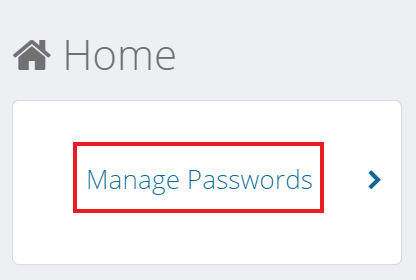
\includegraphics[width=.5\textwidth]{./img/password-1.png}
		\end{figure}
		\vspace{.2cm}
		\begin{figure}
			\centering
			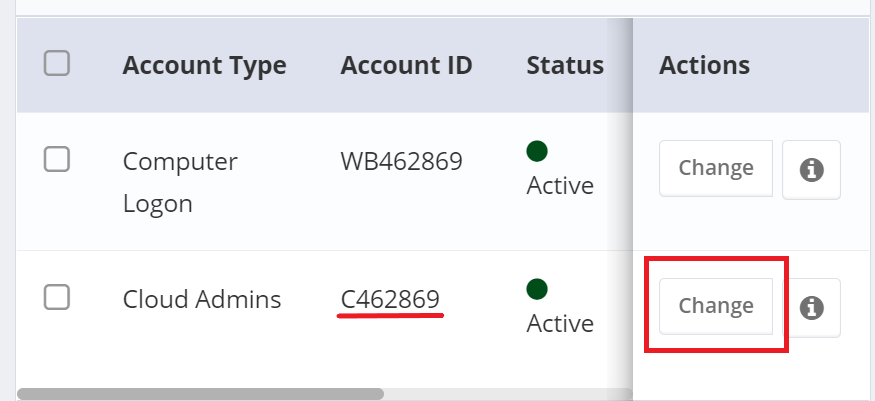
\includegraphics[width=1\textwidth]{./img/password-2.png}
		\end{figure}
		
	\end{columns}
\end{frame}

\begin{frame}
	\frametitle{Manage resource - set-up 2/2}
	\begin{columns}[c]
		
		\column{.650\textwidth} % Right column and width
		
		\begin{enumerate}
			\item Download the \textit{Microsoft Authenticator} app to your smartphone
			\item Go to \url{cloudportal/} on WB intranet
			\item Log in using \textit{c$<$UPI$>$@worldbankgroup.org} (your C-account) and your new password
			\item Click next until you see a QR code - open \textit{Microsoft Authenticator} and scan the QR code
			\item Use code, fingerprint, pattern or similar to approve the authentication in the app
			\item Follow the instructions for how to test the setup, and if success you should see the green check mark and "Notification approved"
			
		\end{enumerate}
		
		\column{.35\textwidth} % Right column and width
		\begin{figure}
			\centering
			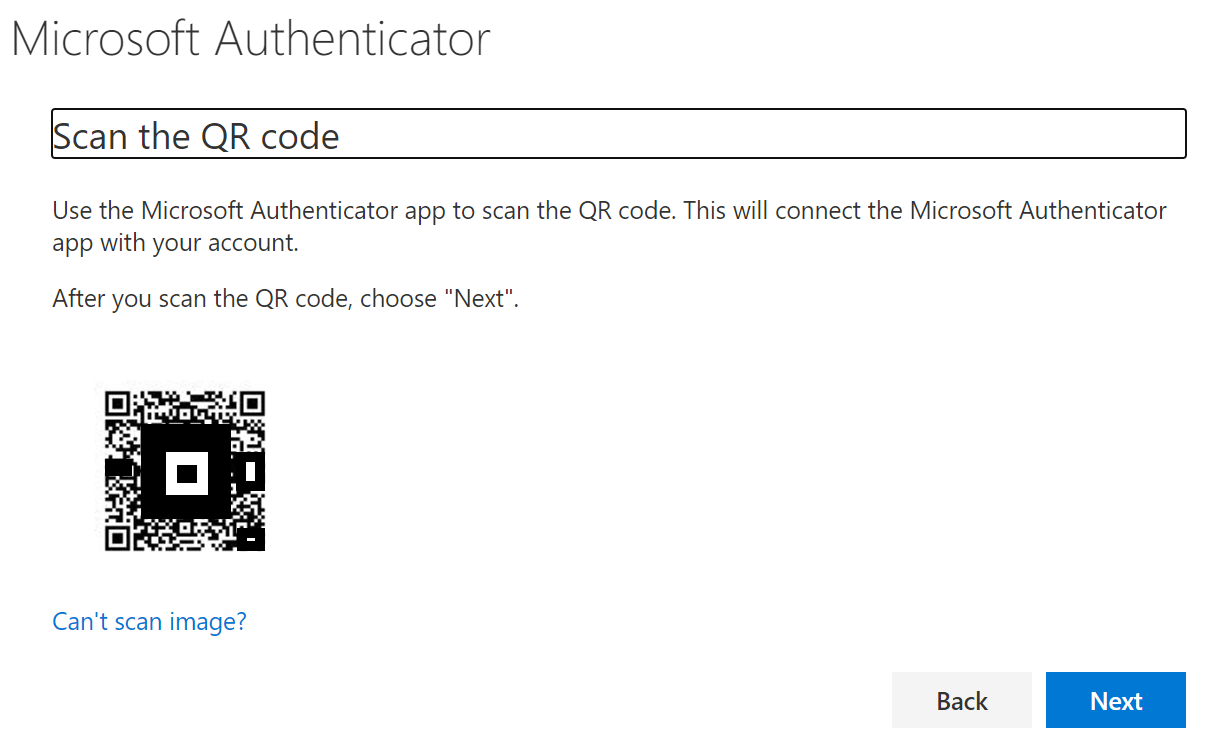
\includegraphics[width=1\textwidth]{./img/microsoft-auth-1.png}
		\end{figure}
			\begin{figure}
			\centering
			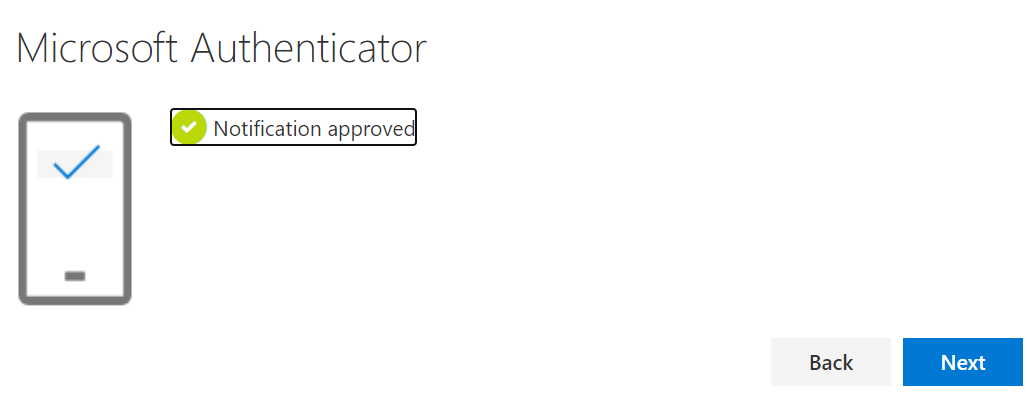
\includegraphics[width=1\textwidth]{./img/microsoft-auth-2.png}
		\end{figure}
			
	\end{columns}
\end{frame}

\begin{frame}
	\frametitle{Manage resource - log on}
	
	
	\begin{columns}[c]
		
		\column{.55\textwidth} % Right column and width
		
		When you are set up, this is how you access the AWS console each time:
		
		\begin{enumerate}
			\item Go to \url{cloudportal/} on WB intranet
			\item Log in using \textit{c$<$UPI$>$@worldbankgroup.org} (your C-account) and your new password
			\item Authenticate with \textit{Microsoft Authenticator}
			\item Click "Amazon web services"
			\item Clikc "AWS Account", then expand (red square) and then click "Management Console"
			
		\end{enumerate}
		
		\column{.45\textwidth} % Right column and width
		\begin{figure}
			\centering
			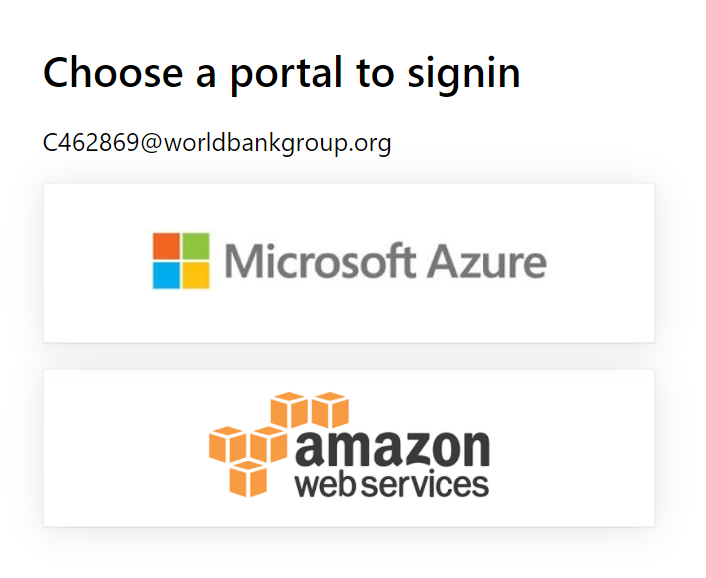
\includegraphics[width=.5\textwidth]{./img/logon-1.png}
		\end{figure}
		\vspace{.2cm}
		\begin{figure}
			\centering
			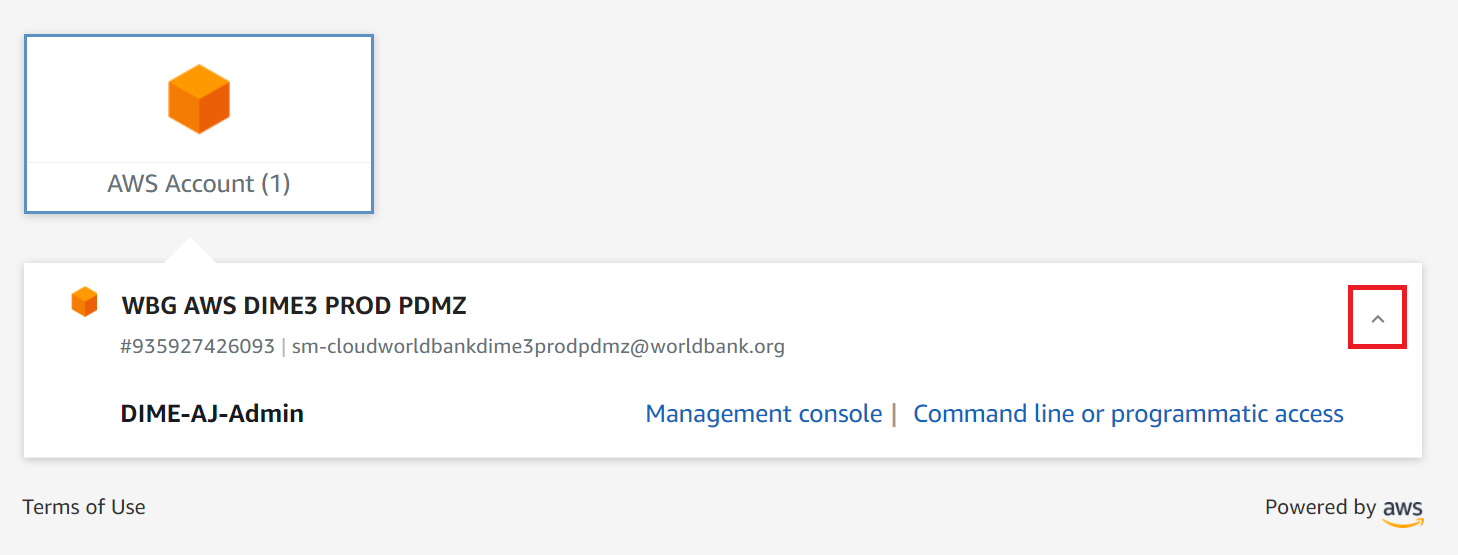
\includegraphics[width=1\textwidth]{./img/logon-2.png}
		\end{figure}
	\end{columns}
\end{frame}


\begin{frame}
	\frametitle{Manage resource - start an EC2 instance}
	
	\begin{columns}[c]
		
		\column{.55\textwidth} % Right column and width
		
		Start an EC2 instance so that you can remote access into it:
			
		\begin{enumerate}
			\item Search for \textit{EC2}
			\item In the menu to the left click \textit{Instances} - see below
			\item Check the instance you want to start - click \textit{Instance state} and select \textit{Start instance}
			\item Refresh until \textit{Pending} turns into \textit{Running}
			
		\end{enumerate}
		
		\begin{figure}
			\centering
			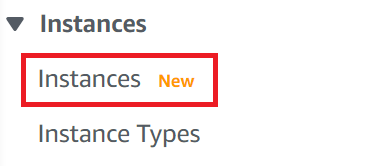
\includegraphics[width=.4\textwidth]{./img/ec2-1.png}
		\end{figure}
		
		
		\column{.45\textwidth} % Right column and width
		\begin{figure}
			\centering
			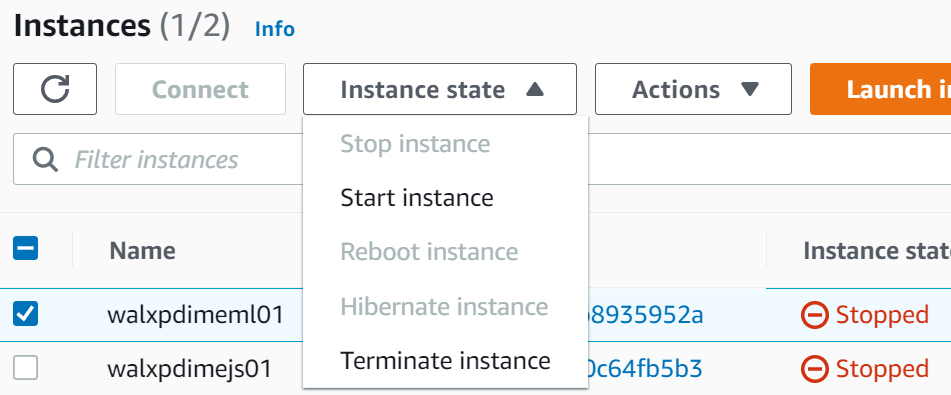
\includegraphics[width=1\textwidth]{./img/ec2-2.png}
		\end{figure}
		\begin{figure}
			\centering
			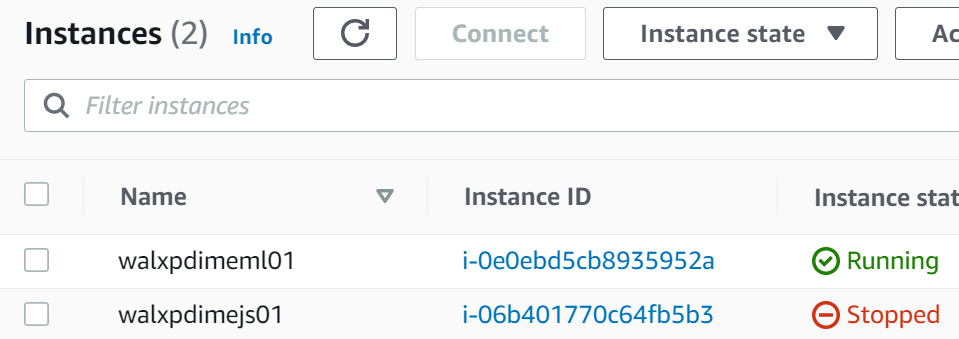
\includegraphics[width=1\textwidth]{./img/ec2-3.png}
		\end{figure}
		\vspace{.5cm}
		
	\end{columns}
\end{frame}


\section{Access WB AWS resources}

\begin{frame}
	\frametitle{WB AWS resource - Access?}
	\begin{columns}[c]
		\column{.50\textwidth} % Left column and width
		\textbf{Access} through the gateway server is both when a resource access the internet and when a resource is accessed from the internet. 
		\vspace{.5cm}\newline
		Examples:
		\begin{itemize}
			%\setlength\itemsep{1em}
			\item Remote in to run a script on an EC2 server
			\item Browsing a shiny app hosted on WB AWS
			\item A script hosted in WB AWS scraped the internet
		\end{itemize}
		
		\column{.50\textwidth} % Right column and width
		\begin{figure}
			\centering
			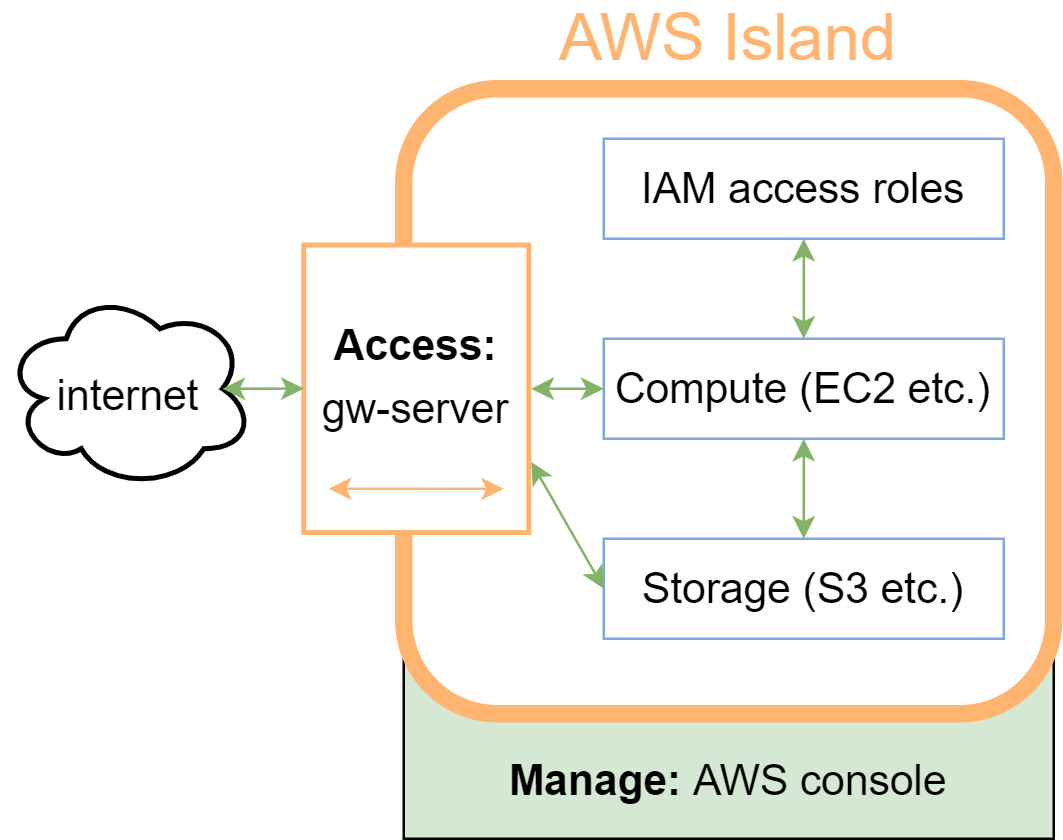
\includegraphics[width=\textwidth]{./img/wb-aws.png}
		\end{figure}
		
	\end{columns}
\end{frame}

\begin{frame}
	\frametitle{Access EC2 resource - run a script}
	\begin{columns}[c]
		\column{.60\textwidth} % Left column and width
		This guide will show you how to access an EC2 instance to run a script
		\begin{itemize}
			%\setlength\itemsep{1em}
			\item Make sure the EC2 instance is started (see previous section)
			\item Open PuTTY on your WB device or WB VDI - self-install from "\textit{Software Center}" if needed
			\item There a many settings, but the only thing you ever need to change is "\textit{Host name}" - set it to either \textit{gw1}, \textit{gw2}, \textit{gw3} or \textit{gw4} - \textit{gw} means "\textit{gateway server}"
			\item Click \textit{Open}
		\end{itemize}
		
		\column{.40\textwidth} % Right column and width
		\begin{figure}
			\centering
			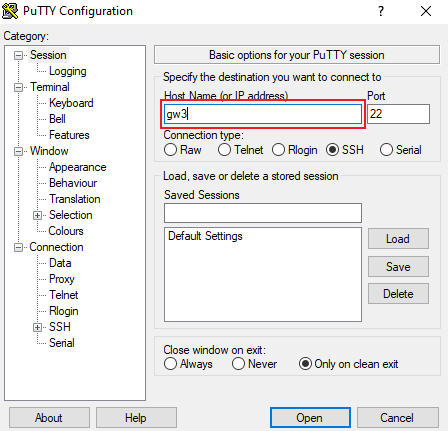
\includegraphics[width=\textwidth]{./img/access-1.png}
		\end{figure}
		
	\end{columns}
\end{frame}

\begin{frame}
	\frametitle{Access EC2 resource - run a script}
	\begin{columns}[c]
		\column{.65\textwidth} % Left column and width
		\begin{itemize}
			%\setlength\itemsep{1em}
			\item Enter your UPI on format \texttt{wb$<$UPI$>$} - press \textit{Enter}
			\item Open your SecureID and enter token for \textit{First Factor} - press \textit{Enter}
			\item Leave \textit{Second Factor} empty - press \textit{Enter}
		\end{itemize}
	
		\begin{figure}
			\centering
			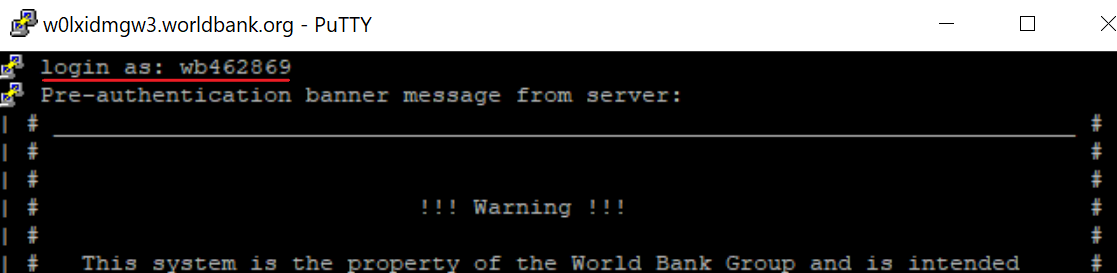
\includegraphics[width=\textwidth]{./img/access-2a.png}
			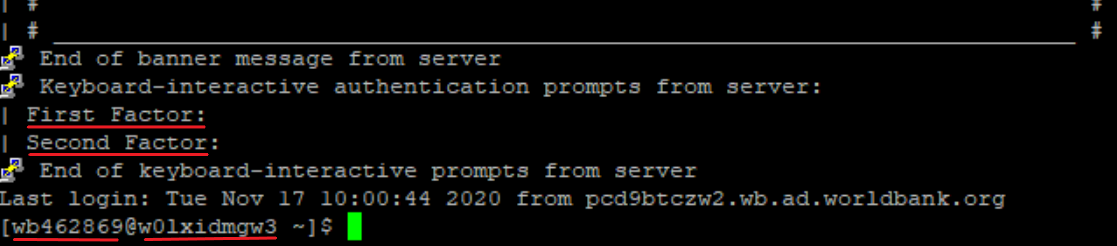
\includegraphics[width=\textwidth]{./img/access-2b.png}
		\end{figure}
		
		\column{.35\textwidth} % Right column and width
		\begin{figure}
			\centering
			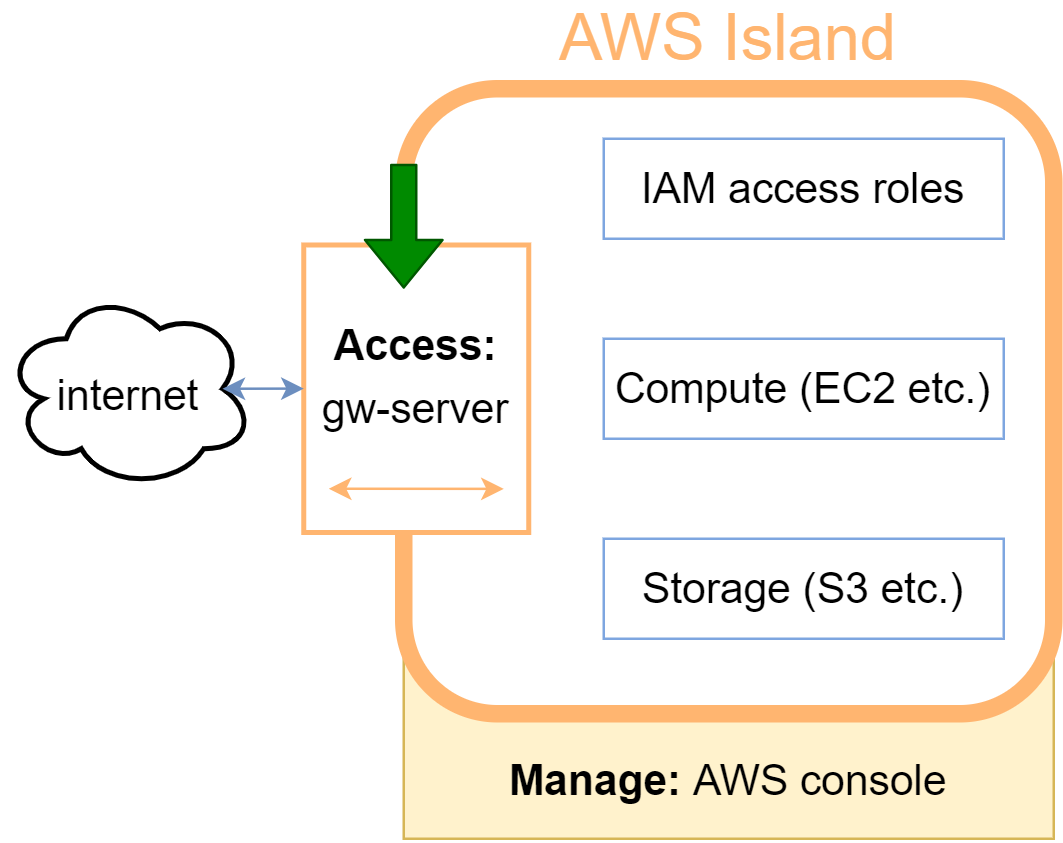
\includegraphics[width=\textwidth]{./img/wb-aws-gw.png}
		\end{figure}
		
	\end{columns}
\end{frame}

\begin{frame}
	\frametitle{Access EC2 resource - run a script}
	\begin{columns}[c]
		\column{.65\textwidth} % Left column and width
		\begin{itemize}
			%\setlength\itemsep{1em}
			\item Now log in to the EC2 server by typing: \newline \texttt{ssh \ectwoName}
		\end{itemize}
		
		\begin{figure}
			\centering
			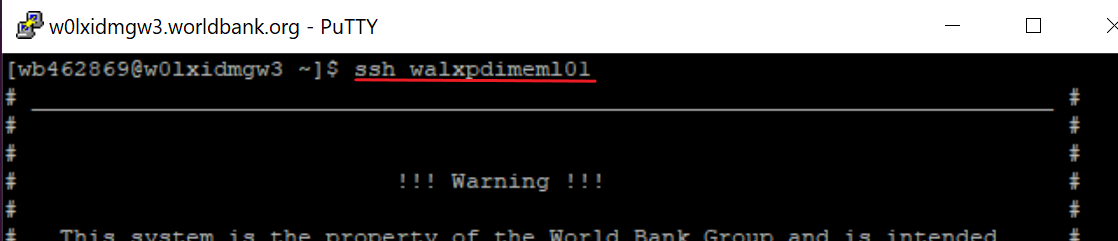
\includegraphics[width=\textwidth]{./img/access-3a.png}
			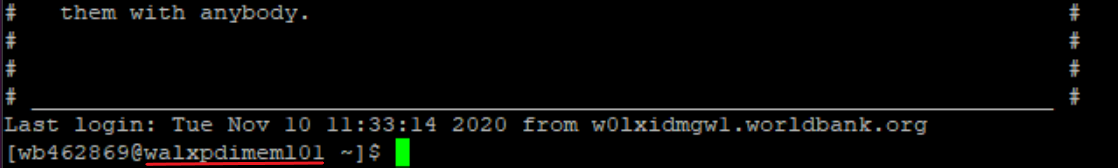
\includegraphics[width=\textwidth]{./img/access-3b.png}
		\end{figure}
		
		\column{.35\textwidth} % Right column and width
		\begin{figure}
			\centering
			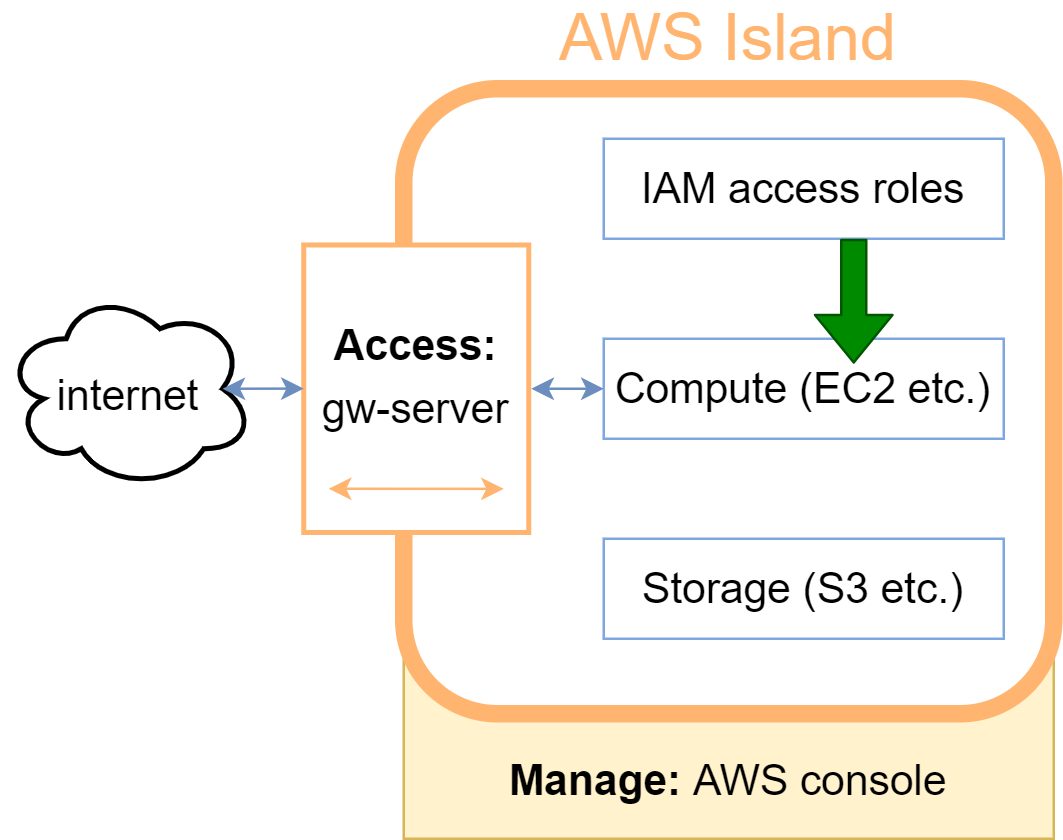
\includegraphics[width=\textwidth]{./img/wb-aws-ec2.png}
		\end{figure}
		
	\end{columns}
\end{frame}

\begin{frame}
	\frametitle{Access EC2 resource - run a script}
	\begin{columns}[c]
		\column{.65\textwidth} % Left column and width
		\begin{itemize}
			%\setlength\itemsep{1em}
			\item Now get full access by updating your user role to your team's user role: \newline \texttt{sudo su - \srvAcctName}
		\end{itemize}
		
		\begin{figure}
			\centering
			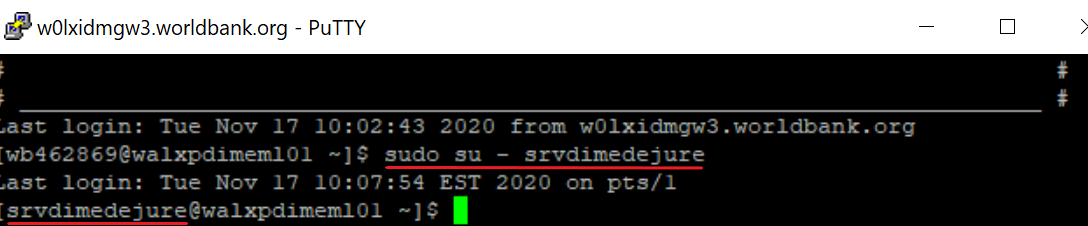
\includegraphics[width=\textwidth]{./img/access-4.png}
		\end{figure}
		
		\column{.35\textwidth} % Right column and width
		\begin{figure}
			\centering
			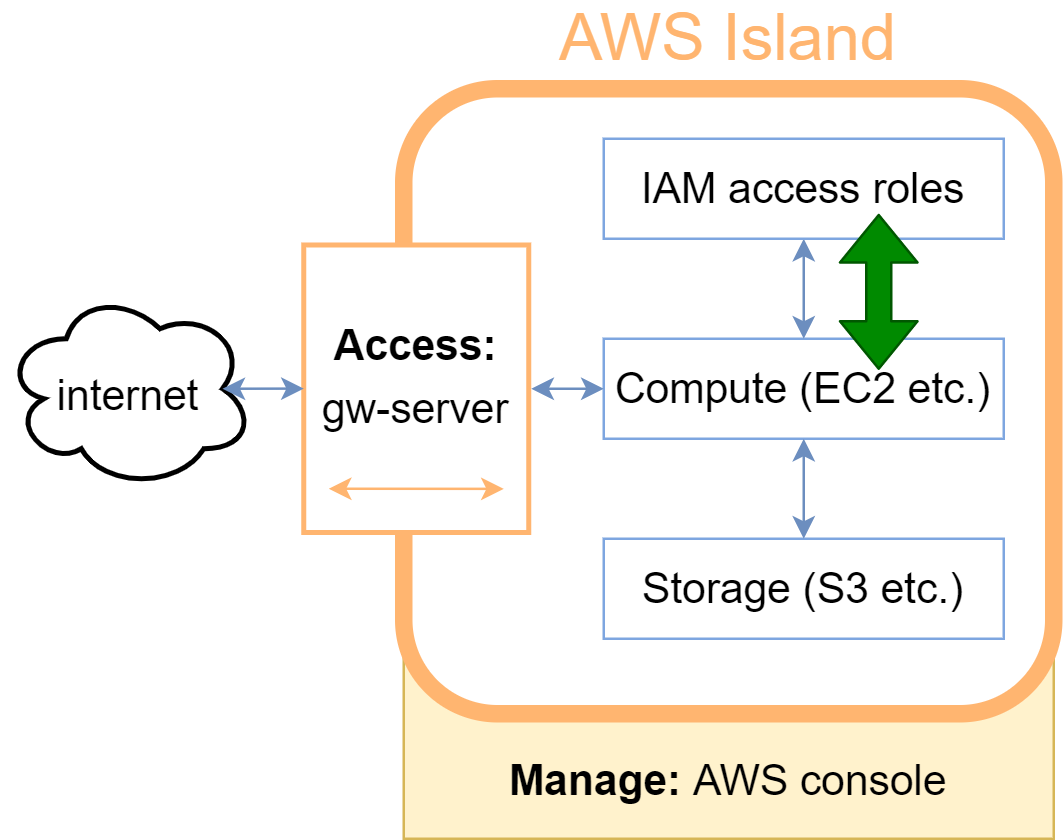
\includegraphics[width=\textwidth]{./img/wb-aws-iam.png}
		\end{figure}
		
	\end{columns}
\end{frame}

\begin{frame}
	\frametitle{Access EC2 resource - run a script}
	\vspace{1cm}
	\begin{columns}[c]
		\column{.45\textwidth} % Left column and width
		Now lets run a test script:
		\begin{itemize}
			\item Navigate into the test folder:
			\begin{itemize}
				\item \texttt{cd GitHub}
				\item \texttt{cd test}
			\end{itemize}
			\item Run the test script:
			\begin{itemize}
				\item \texttt{python test-access.py}
			\end{itemize}
		\end{itemize}
		
		\column{.55\textwidth} % Right column and width
		\begin{figure}
			\centering
			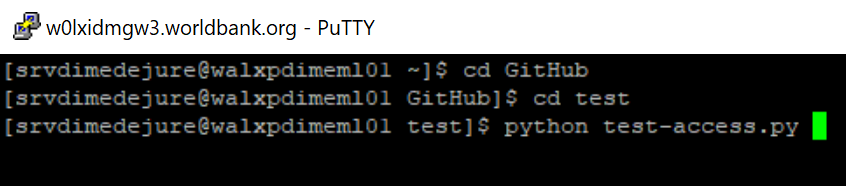
\includegraphics[width=\textwidth]{./img/access-5.png}
		\end{figure}
		
	\end{columns}
	
	\vspace{1cm}
	\small (You can of course run the script from the home folder by typing: \newline \texttt{python GitHub/test/test-access.py} - but you will soon learn what your preference is)

\end{frame}

\section{WB AWS best practices}

\end{document}
